\documentclass[mathserif]{beamer}

\usepackage{microtype}
\usepackage{xparse}
\usepackage{amsmath}
\usepackage{amssymb}
\usepackage{mathtools}
\usepackage{graphicx}

\frenchspacing

\logo{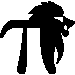
\includegraphics[width=0.07\textwidth]{../Logo}}

\usetheme{Rochester}
\usecolortheme{whale}

\setbeamertemplate{frametitle continuation}[from second][\hfill\insertcontinuationtext]

% Table of contents at start of each section
\AtBeginSection[] {%
	\begin{frame}
		\frametitle{Table of Contents}
		\tableofcontents[currentsection]
	\end{frame}
}

% Environments for math
\newenvironment{compactmath}[1][\normalsize]%
	{\begin{minipage}{\textwidth}\vspace{-0.5\baselineskip}#1\begin{equation*}}
	{\end{equation*}\end{minipage}}

\newenvironment{sizedmath}[1]%
	{\begingroup#1\begin{equation*}}
	{\end{equation*}\endgroup}

% Environments for consistent frame use
\newenvironment{namedframe}[1]%
	{\begin{frame}\frametitle{#1}\framesubtitle{\secname}}
	{\end{frame}}

\newenvironment{namedbreakframe}[1]%
	{\begin{frame}[allowframebreaks]\frametitle{#1}\framesubtitle{\secname}}
	{\end{frame}}

% Frames for emphasis
\newcommand{\sectionstart}[2]{\begin{frame}\frametitle{#1}\centering\Huge\secname\\\Large#2\end{frame}}
\newcommand{\bigframe}[1]{\begin{namedframe}{#1}\Huge\centering#1\end{namedframe}}

% Spacing commands
\newcommand{\sep}{\\\pause\vspace{1ex}}
\newcommand{\varsep}[1]{\\\pause\vspace{#1}}

\newcommand{\vertspace}{\\\vspace{1ex}}
\newcommand{\varvertspace}[1]{\\\vspace{#1}}

% Text formatting
\DeclareTextFontCommand{\emph}{\bfseries}

% Macros for math
\newcommand{\such}{\ |\ }
\DeclarePairedDelimiter{\ceil}{\lceil}{\rceil}
\DeclarePairedDelimiter{\floor}{\lfloor}{\rfloor}


\usepackage{mathtools}

\usepackage{tikz}

\newenvironment{explodingdots}[1]%
	{\begin{center}\begin{tikzpicture}\draw[step=2cm,black,thick] (0,0) grid(2 * #1,2);}
	{\end{tikzpicture}\end{center}}

\tikzset{dot/.style= {circle,fill=black,draw,scale=0.75}}
\tikzset{tod/.style= {circle,fill=none,draw,scale=0.75}}
\tikzset{explode/.style= {circle,fill=red,draw,minimum size=1.75cm}}

\newcommand{\mach}[2]{#2 \leftarrow #1}
\newcommand{\textmach}[2]{$#2 \leftarrow #1$}

%  longdiv.tex  v.1  (1994)  Donald Arseneau  
%
%  Work out and print integer long division problems.  Use:
%       \longdiv{numerator}{denominator}
%  The numerator and denominator (divisor and dividend) must be integers, and
%  the quotient is an integer too.  \longdiv leaves a remainder.
%  Use this in any type of TeX.

\newcount\gpten % (global) power-of-ten -- tells which digit we are doing
\countdef\rtot2 % running total -- remainder so far
\countdef\LDscratch4 % scratch

\def\longdiv#1#2{%
 \vtop{\normalbaselines \offinterlineskip
   \setbox\strutbox\hbox{\vrule height 2.1ex depth .5ex width0ex}%
   \def\showdig{$\underline{\the\LDscratch\strut}$\cr\the\rtot\strut\cr
       \noalign{\kern-.2ex}}%
   \global\rtot=#1\relax
   \count0=\rtot\divide\count0by#2\edef\quotient{\the\count0}%\show\quotient
   % make list macro out of digits in quotient:
   \def\temp##1{\ifx##1\temp\else \noexpand\dodig ##1\expandafter\temp\fi}%
   \edef\routine{\expandafter\temp\quotient\temp}%
   % process list to give power-of-ten:
   \def\dodig##1{\global\multiply\gpten by10 }\global\gpten=1 \routine
   % to display effect of one digit in quotient (zero ignored):
   \def\dodig##1{\global\divide\gpten by10
      \LDscratch =\gpten
      \multiply\LDscratch  by##1%
      \multiply\LDscratch  by#2%
      \global\advance\rtot-\LDscratch \relax
      \ifnum\LDscratch>0 \showdig \fi % must hide \cr in a macro to skip it
   }%
   \tabskip=0pt
   \halign{\hfil##\cr % \halign for entire division problem
     $\quotient$\strut\cr
     #2$\,\overline{\vphantom{\big)}%
     \hbox{\smash{\raise3.5\fontdimen8\textfont3\hbox{$\big)$}}}%
     \mkern2mu \the\rtot}$\cr\noalign{\kern-.2ex}
     \routine \cr % do each digit in quotient
}}}

\endinput % Demonstration below:

\noindent Here are some long division problems

\indent
\longdiv{12345}{13} \quad
\longdiv{123}{1234} \quad
\longdiv{31415926}{2} \quad
\longdiv{81}{3} \quad
\longdiv{1132}{99} \quad
\longdiv{86491}{94}
\bye


\frenchspacing

\title{James Tanton's Exploding Dots}
\author{Vincent Macri}
\date{
\includegraphics{by-nc-sa}\\\copyright{} Vincent Macri, 2017\\\footnotesize\url{https://creativecommons.org/licenses/by-nc-sa/4.0/}}


\newenvironment{whatif}%
	{\begin{namedframe}{What if\ldots}\Huge What if\ldots\normalsize

	}
	{\end{namedframe}}

\newcommand{\bigframe}[1]{\begin{namedframe}{#1}\Huge\centering#1\end{namedframe}}

\begin{document}
	\frame{\titlepage}
	\section{Mechania}
\begin{namedframe}{The \textmach{1}{2} machine}
	\only<1>{
		\begin{explodingdots}{2}
			\draw (3.5,1) node[dot]{};
			\draw (2.5,1) node[dot]{};
		\end{explodingdots}
	}
	\only<2>{
		\begin{explodingdots}{2}
			\draw (3,1) node[explode]{Boom!};
		\end{explodingdots}
	}
	\only<3>{
		\begin{explodingdots}{2}
			\draw (1,1) node[dot]{};
		\end{explodingdots}
	}
\end{namedframe}
\begin{namedframe}{\textmach{1}{2} examples}
	What are the following in a \textmach{1}{2} machine?
	\begin{description}
		\item[$1$] $\xrightarrow{\mach{1}{2}}$ \visible<2->{$1$}
		\item[$2$] $\xrightarrow{\mach{1}{2}}$ \visible<3->{$10$}
		\item[$3$] $\xrightarrow{\mach{1}{2}}$ \visible<4->{$11$}
		\item[$4$] $\xrightarrow{\mach{1}{2}}$ \visible<5->{$100$}
		\item[$5$] $\xrightarrow{\mach{1}{2}}$ \visible<6->{$101$}
		\item[$13$] $\xrightarrow{\mach{1}{2}}$ \visible<7->{$1101$}
	\end{description}
\end{namedframe}
\begin{whatif}
	What if we had a \textmach{1}{3} machine?
\end{whatif}
\begin{whatif}
	What if we had a \textmach{1}{10} machine?
\end{whatif}

	\section{Insighto}
\begin{namedframe}{What are these machines?}
	These machines are another way of handling arithmetic, but they work in any base.

	A \textmach{1}{b} machine handles numbers in base $b$.

	We'll use a \textmach{1}{10} machine for now.
\end{namedframe}

	\section{Arithmos}
\begin{namedframe}{What next?}
	We can count with these machines, but what else can we do?

	\pause
	What's the first thing you learn to do with numbers after counting?
\end{namedframe}
\bigframe{Addition!}
\begin{namedframe}{Examples}
	What is $234 + 125$?
	\pause
	\begin{equation*}
		\begin{array}{rrrr}
			  & 2 & 3 & 4\\
			+ & 1 & 2 & 5\\\hline
			  & 3 & 5 & 9
		\end{array}
	\end{equation*}
	\pause
	What is $234 + 187$?
	\pause
	\begin{equation*}
		\begin{array}{rrrr}
			  & 2 & 3  & 4\\
			+ & 1 & 8  & 7\\\hline
			  & 3 & 11 & 11
		\end{array}
	\end{equation*}
	\pause
	Three hundred eleventy eleven!

	But now society thinks I'm weird. Let's fix that.
\end{namedframe}
\begin{namedframe}{Explode the dots!}
	Three hundred eleventy eleven in a \textmach{1}{10} machine.
	\only<1>{
		\begin{explodingdots}{3}
			\draw (1,0.5) node[dot]{};
			\draw (1,1) node[dot]{};
			\draw (1,1.5) node[dot]{};

			\draw (2.25,0.25) node[dot]{};
			\draw (2.5,0.75) node[dot]{};
			\draw (2.5,1.25) node[dot]{};
			\draw (2.5,1.75) node[dot]{};
			\draw (3,0.25) node[dot]{};
			\draw (3,0.75) node[dot]{};
			\draw (3,1.25) node[dot]{};
			\draw (3,1.75) node[dot]{};
			\draw (3.5,0.5) node[dot]{};
			\draw (3.5,1) node[dot]{};
			\draw (3.5,1.5) node[dot]{};

			\draw (4.5,0.25) node[dot]{};
			\draw (4.5,0.75) node[dot]{};
			\draw (4.5,1.25) node[dot]{};
			\draw (4.5,1.75) node[dot]{};
			\draw (5,0.25) node[dot]{};
			\draw (5,0.75) node[dot]{};
			\draw (5,1.25) node[dot]{};
			\draw (5,1.75) node[dot]{};
			\draw (5.5,0.5) node[dot]{};
			\draw (5.5,1) node[dot]{};
			\draw (5.5,1.5) node[dot]{};
		\end{explodingdots}
	}
	\only<2>{
		\begin{explodingdots}{3}
			\draw (1,0.5) node[dot]{};
			\draw (1,1) node[dot]{};
			\draw (1,1.5) node[dot]{};
			\draw (1.5,1.5) node[dot]{};

			\draw (3,1) node[explode]{Boom!};
			\draw (2.25,0.25) node[dot]{};

			\draw (4.5,0.25) node[dot]{};
			\draw (4.5,0.75) node[dot]{};
			\draw (4.5,1.25) node[dot]{};
			\draw (4.5,1.75) node[dot]{};
			\draw (5,0.25) node[dot]{};
			\draw (5,0.75) node[dot]{};
			\draw (5,1.25) node[dot]{};
			\draw (5,1.75) node[dot]{};
			\draw (5.5,0.5) node[dot]{};
			\draw (5.5,1) node[dot]{};
			\draw (5.5,1.5) node[dot]{};
		\end{explodingdots}
	}
	\only<3>{
		\begin{explodingdots}{3}
			\draw (1,0.5) node[dot]{};
			\draw (1,1) node[dot]{};
			\draw (1,1.5) node[dot]{};
			\draw (1.5,1.5) node[dot]{};

			\draw (2.25,0.25) node[dot]{};

			\draw (4.5,0.25) node[dot]{};
			\draw (4.5,0.75) node[dot]{};
			\draw (4.5,1.25) node[dot]{};
			\draw (4.5,1.75) node[dot]{};
			\draw (5,0.25) node[dot]{};
			\draw (5,0.75) node[dot]{};
			\draw (5,1.25) node[dot]{};
			\draw (5,1.75) node[dot]{};
			\draw (5.5,0.5) node[dot]{};
			\draw (5.5,1) node[dot]{};
			\draw (5.5,1.5) node[dot]{};
		\end{explodingdots}
	}
	\only<4>{
		\begin{explodingdots}{3}
			\draw (1,0.5) node[dot]{};
			\draw (1,1) node[dot]{};
			\draw (1,1.5) node[dot]{};
			\draw (1.5,1.5) node[dot]{};

			\draw (2.25,0.25) node[dot]{};
			\draw (2.5,1) node[dot]{};

			\draw (5,1) node[explode]{Boom!};
			\draw (5.5,0.5) node[dot]{};
		\end{explodingdots}
	}
	\only<5>{
		\begin{explodingdots}{3}
			\draw (1,0.5) node[dot]{};
			\draw (1,1) node[dot]{};
			\draw (1,1.5) node[dot]{};
			\draw (1.5,1.5) node[dot]{};

			\draw (2.25,0.25) node[dot]{};
			\draw (2.5,1) node[dot]{};

			\draw (5.5,0.5) node[dot]{};
		\end{explodingdots}
	}
	\visible<5->{
		\[421\]
	}
\end{namedframe}
\bigframe{What do we learn after addition?}
\bigframe{Multiplication!}
\begin{namedframe}{Examples}
	What is $2876 \times 3$?
	\begin{equation*}
		\begin{array}{rrrr}
			2 & 8 & 7 & 6\\
			\times & & & 3\\\hline
			6 & 24 & 21 & 18
		\end{array}
	\end{equation*}
	Let's fix this one together for society.
	\Huge
	\begin{explodingdots}{4}
		\draw (1,1) node{6};
		\draw (3,1) node{24};
		\draw (5,1) node{21};
		\draw (7,1) node{18};
	\end{explodingdots}
\end{namedframe}

	\section{Antidotia}
\begin{namedframe}{Subtraction}
	\begin{alertblock}{Theorem 1}
		Subtraction does not exist.
	\end{alertblock}
	\begin{alertblock}{Theorem 2}
		What we call subtraction is just the addition of negative numbers.

		Or, subtraction is the addition of the opposite.
	\end{alertblock}
\end{namedframe}
\begin{namedframe}{The antidot}
	The opposite of a dot is an antidot. I'll call these tods.

	This is one tod in one of our machines:
	\begin{explodingdots}{1}
		\draw (1,1) node[tod]{};
	\end{explodingdots}
\end{namedframe}
\begin{namedframe}{How do tods behave?}
	\only<1>{
		\begin{explodingdots}{1}
			\draw (1,1.5) node[dot]{};
			\draw (1,0.5) node[tod]{};
		\end{explodingdots}
	}
	\only<2>{
		\begin{explodingdots}{1}
			\draw (1,1) node[explode]{Poof!};
		\end{explodingdots}
	}
	\only<3>{
		\begin{explodingdots}{1}
		\end{explodingdots}
	}
\end{namedframe}
\begin{namedframe}{Examples}
	What is $564 - 123$?
	\pause
	\begin{equation*}
		\begin{array}{rrrr}
			  & 5 & 6 & 4\\
			- & 1 & 2 & 3\\\hline
			  & 4 & 4 & 1
		\end{array}
	\end{equation*}
	\pause
	What is $441 - 254$?
	\pause
	\begin{equation*}
		\begin{array}{rrrr}
			  & 4 & 4 & 1\\
			- & 2 & 5 & 4\\\hline
			  & 2 & -1 & -3
		\end{array}
	\end{equation*}
	\pause
	Let's fix this together on the board for society's sake. We'll use the exploding dots method.
\end{namedframe}
\begin{namedframe}{Another method}
	\begin{explodingdots}{3}
		\draw (0.5,1) node[dot]{};
		\draw (1.5,1) node[dot]{};

		\draw (3,1) node[tod]{};

		\draw (5,1.5) node[tod]{};
		\draw (5,1) node[tod]{};
		\draw (5,0.5) node[tod]{};
	\end{explodingdots}
	\pause
	There is another way to fix this which is helpful for doing math mentally.

	\pause
	Let's look the place values:
	\[200 + -10 + -3\]

	\pause
	This is very easy to do mentally.

	\[200 + -10 = 190 + -3\]
	\[190 + -3 = 187\]
\end{namedframe}

	\section{Obelus}
\begin{namedframe}{Division}
	Fun fact before we get started on division, did you know that the $\div$ sign is called an obelus?
\end{namedframe}
\begin{namedframe}{Long division method}
	What is $276 \div 12$?

	\alert{Don't use a calculator!}
	\pause
	{\rmfamily
	\begin{equation*}
		\longdiv{276}{12}
	\end{equation*}
	}
	This is stupid and convoluted. Let's use exploding dots instead.
\end{namedframe}
\begin{namedframe}{Exploding dots method}
	\[276 \div 12\]
	$276$:
	\begin{explodingdots}{3}
		\draw (0.5,1) node[dot]{};
		\draw (1.5,1) node[dot]{};

		\draw (2.5,0.5) node[dot]{};
		\draw (2.5,1) node[dot]{};
		\draw (2.5,1.5) node[dot]{};
		\draw (3.5,0.5) node[dot]{};
		\draw (3.5,1) node[dot]{};
		\draw (3.5,1.5) node[dot]{};
		\draw (3,1) node[dot]{};

		\draw (4.5,0.5) node[dot]{};
		\draw (4.5,1) node[dot]{};
		\draw (4.5,1.5) node[dot]{};
		\draw (5.5,0.5) node[dot]{};
		\draw (5.5,1) node[dot]{};
		\draw (5.5,1.5) node[dot]{};
	\end{explodingdots}
	$12$:
	\begin{explodingdots}{2}
		\draw (1,1) node[dot]{};

		\draw (3,0.5) node[dot]{};
		\draw (3,1.5) node[dot]{};
	\end{explodingdots}
	Let's look for groups of $12$ in $276$.
\end{namedframe}
\begin{namedframe}{Exploding dots solution}
	\begin{explodingdots}{2}
		\draw (1,1) node[dot]{};

		\draw (3,0.5) node[dot]{};
		\draw (3,1.5) node[dot]{};
	\end{explodingdots}
	\pause
	\begin{explodingdots}{3}
		\draw (0.5,1) node[dot,red]{};
		\draw (1.5,1) node[dot,green]{};

		\draw (3,2.5) node{\Huge $2$};
		\draw (2.5,0.5) node[dot,red]{};
		\draw (2.5,1) node[dot,red]{};
		\draw (2.5,1.5) node[dot,green]{};
		\draw (3.5,0.5) node[dot,green]{};
		\draw (3.5,1) node[dot,blue]{};
		\draw (3.5,1.5) node[dot,yellow]{};
		\draw (3,1) node[dot,orange]{};

		\draw (5,2.5) node{\Huge $3$};
		\draw (4.5,0.5) node[dot,blue]{};
		\draw (4.5,1) node[dot,blue]{};
		\draw (4.5,1.5) node[dot,yellow]{};
		\draw (5.5,0.5) node[dot,yellow]{};
		\draw (5.5,1) node[dot,orange]{};
		\draw (5.5,1.5) node[dot,orange]{};
	\end{explodingdots}
	\pause
	\[273 \div 12 = 23\]
\end{namedframe}
\begin{namedframe}{Examples together}
What is $2783 \div 23$?
\pause
$121$

\pause
What is $2785 \div 23$?
\pause
$121\ \text{R}2$ or $121 + \frac{2}{23}$
\end{namedframe}

	\section{Eks}
\begin{whatif}
	What if we had a \textmach{x}{1} machine? What would it look like?
	\pause
	\begin{explodingdots}{5}
		\draw (1,-0.5) node{\Huge $x^4\vphantom{x^4}$};
		\draw (3,-0.5) node{\Huge $x^3\vphantom{x^4}$};
		\draw (5,-0.5) node{\Huge $x^2\vphantom{x^4}$};
		\draw (7,-0.5) node{\Huge $x\vphantom{x^4}$};
		\draw (9,-0.5) node{\Huge $1\vphantom{x^4}$};
	\end{explodingdots}
	\pause
	With this knowledge, we can now manipulate polynomials just like we do regular numbers.
\end{whatif}
\begin{namedframe}{Polynomial division}
	What is $\displaystyle\frac{2x^2 + 7x + 6}{x+2}$? \pause\hspace{1ex}$2x + 3$

	\pause
	What is $\displaystyle\frac{x^4 + 2x^3 + 4x^2 + 6x + 3}{x^2+3}$? \pause\hspace{1ex} $x^2 + 2x + 1$

	\pause

	What is $\displaystyle\frac{x^3 - 3x + 2}{x+2}$? \pause\hspace{1ex} $x^2 - 2x + 1$
\end{namedframe}

	\section{Infinitia}
\begin{namedframe}{Now it gets \emph{really} fun}
	\Huge
	\[\frac{1}{1-x}\]
\end{namedframe}
\begin{namedframe}{Geometric series formula}
	Using dots and boxes, we get what is knows at the \alert{geometric series formula}:
	\pause
	\[1 + x + x^2 + x^3 + x^4 + x^5 + x^6 + x^7 + x^8 + x^9 \dots\]
	\pause
	In calculus, we would call this the \alert{Taylor series} of $\frac{1}{1-x}$.
\end{namedframe}
\begin{namedframe}{This is really cool}
	Using the dots and boxes method, find the Taylor series of:
	\Huge
	\[\frac{1}{1-x-x^2}\]
\end{namedframe}

	\begin{frame}
		\frametitle{Congratulations!}
		We just went from kindergarten arithmetic to advanced calculus in 40 minutes!
	\end{frame}
\end{document}
